\documentclass[10pt, a4paper]{article}
\usepackage{polski}
\usepackage[polish]{babel}
\usepackage[utf8]{inputenc}
\usepackage{outline}
\usepackage{pmgraph}
\usepackage[normalem]{ulem}
\usepackage{graphicx} 
\usepackage{booktabs} 

\title{\vspace{175pt}\textbf{Wizualizacja pogody w Polsce\\}  \small{\vspace{10pt}Wizualizacja danych sensorycznych}}
\author{Cyprian Hryniuk}
\date{\oldstylenums{20}/\oldstylenums{03}/\oldstylenums{19}}
%--------------------Make usable space all of page
\setlength{\oddsidemargin}{0in}
\setlength{\evensidemargin}{0in}
\setlength{\topmargin}{0in}
\setlength{\headsep}{-.25in}
\setlength{\textwidth}{6.5in}
\setlength{\textheight}{8.5in}
%--------------------Indention
\setlength{\parindent}{1cm}

\begin{document}
%--------------------Title Page
\begin{titlepage}
\maketitle
\thispagestyle{empty}
\end{titlepage}

\newpage
\tableofcontents
\newpage
\section{Opis projektu}
\label{sec:opisprojektu}
\indent

Projekt ma na celu stworzenie aplikacji okienkowej wizualizującej dane uzyskane z witryny internetowej dotyczące pogody na terenie Polski. Wizualizacji podlegać będą dane historyczne, aktualne oraz prognoza. Dla terenu Polski przetwarzane dane będą dotyczyć temperatury oraz opadów, a dla większych miast (Warszawa, Wrocław, Kraków, Łódź, Poznań, Katowice, Gdańśk) temperatury, opadów, ciśnienia i siły wiatru. 

Wszystkie dokumenty dotyczące projektu będą tworzone w systemie \LaTeX. Całość projektu przechowywana będzie w zdalnym repozytorium w serwisie internetowym github.com, a dokumentacja tworzona będzie generatorem doxygen. 

\subsection{Przewidziane funkcjonalności}
\label{ssec:funkc}
\begin{itemize}
  \item Zbieranie danych dotyczących pogody oraz jej prognozy z odpowiednich serwisów internetowych.
  \item Przechowywanie i animowane wizualizowanie historii, akutalnej i prognozy pogody dla terenu całej Polski oraz dokładniejszych inforamcji dla większych miast.
  \item Użytkownik będzie miał możliwość przęłączania się pomiędzy wizualizacją pogody dla wybranego terminu (historię/aktualną/prognozę). 
  \item Użytkownik będzie miał możliwość przełączania się międzya wizualizacją pogody dla terenu całej Polski albo dla wybranego miasta.
  
\end{itemize}

\section{Harmonogram}
\label{sec:harmonogram}
\subsection{Wykres Gantta}
    \begin{figure}[h]
    \centering
	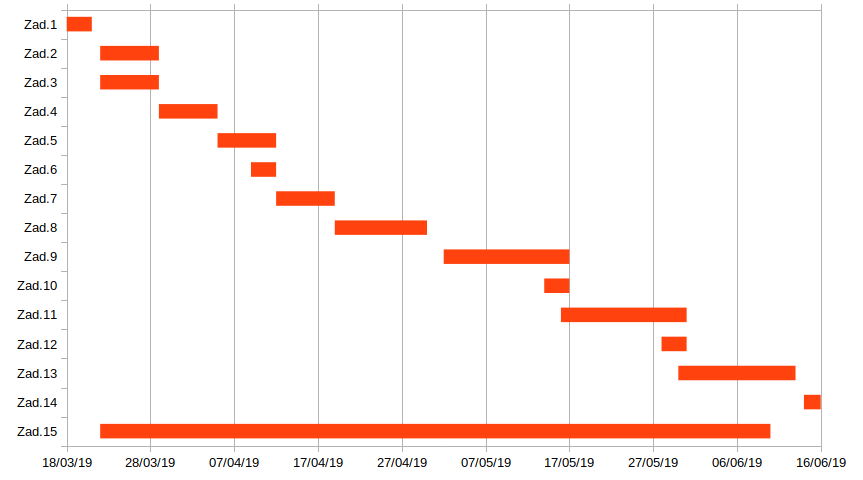
\includegraphics[width=0.94\textwidth]{wizualizacja_gantt.png}
	\caption{Wykres Gantta}
\end{figure}
\newpage
\subsection{Spis zadań}
\begin{table}[!h]
	\centering
	\caption{Harmonogram zadań}
	\label{table_exres}
	\begin{tabular}{p{20mm}p{120mm}}
		\toprule
		termin & opis\\ \midrule
		18.03 -- 22.03 & 1. Określenie wymagań użytkownika, funkcjonalności, dekompozycja problemu  \\
		\midrule
		22.03 - 28.03 & 2. Wstępny projekt interfejsu graficznego stworzonego w QtDesignerze. \newline 3. Zebranie odpowiednich grafik potrzebnych do stworzenia aplikacji okienkowej.\\
		\midrule
	    29.03 - 4.04 & 4. Pobieranie danych z serwisów internetowych, przetworzenie ich oraz zapis do plików tekstowych przechowujących zebrane dane. \\
		\midrule
		 5.04 - 11.04 & 5. Wstępna wizualizacja danych pogodowych - dla aktualnej pogody - obszar Polski. \newline 6. Sporządzenie raportu wstępnego.\\
		 \midrule
        12.04 - 18.04 &  7. Wstępna wizualizacja danych pogodowych - dla aktualnej pogody - wybrane miasta.\\

		\midrule
        19.04 - 1.05 & 8. Wstępna wizualizacja danych pogodowych - historia oraz prognoza pogody - obszar Polski. \\ 

		\midrule
        2.05 - 16.05 & 9. Wstępna wizualizacja danych pogodowych - historia oraz prognoza pogody - wybrane miasta. \newline 10. Sporządzenie raportu rezultatów zaawansowanych. \\

		\midrule
        16.05 - 30.05 & 11. Dopracowanie wizualizacji danych pogodowych - animacja. \newline 12. Sporządzenie raportu rezultatów prawie końcowych. \\
        
        \midrule 
        30.05 - 16.06 & 13. Dopracowanie interfejsu graficznego, optymalizacja kodu. 
        \newline 14. Sporządzenie raportu końcowego. \\
        \midrule
        22.03 - 15.06 & 15. Tworzenie dokumentacji w doxygenie. \\

		\bottomrule
	\end{tabular}
\end{table}

\subsection{Kamienie milowe}
   \begin{table}[!h]
	\label{table_exres}
	\begin{tabular}{p{15mm}|p{120mm}}
		
		termin & kamień milowy\\ \hline
		11.04 & wstępna wizualizacja aktualnych danych pogodowych dla terenu Polski - wymaga zaimplementowanego pobierania i przechowywania danych, a także projektu graficznego aplikacji\\

		16.05 & zrealizowanie wszystkich wstępnych wizualizacji dostępnych w aplikacji - dla obszaru całej Polski, a także dla większych miast wizualizacja historii, aktualnej oraz prognozy pogody\\
	\end{tabular}
	\caption{Kamienie milowe}
\end{table}



\end{document}
